\chapter{Funções exponenciais e logarítmicas}
 \section{Funções exponenciais}

  \colorbox{azul}{
 \begin{minipage}{0.9\linewidth}
 \begin{center}
 São funções $f: \R \rightarrow \R_{+}^{*} $ tais que:
 \[f(x) = a^x\]
 onde é dado $a \in \R_{+}$ satisfazendo $0 < a$ e $a \neq 1$. Estas funções são chamadas funções exponenciais de base $a$.
 \end{center}
 \end{minipage}}
 \vskip0.3cm

 Observe que:
 \begin{itemize}
  \item exigimos que a constante $a$ fosse positiva para garantir que a função estivesse definida para todo $x$ real (lembre-se que, por exemplo, $\sqrt{a}= a^{\frac{1}{2}}$ não está definida para $a$ negativo);
  \item excluímos $a=1$, pois $1^x=1$ para todo $x$ real, de modo que $f(x)= 1^x$ é uma função constante.
 \end{itemize}

 \begin{exem}\label{ex:exp-2}
  Considere a função $f: \R \rightarrow \R_{+}^{*} $ dada por,
  \[f(x) = 2^x \ , \]
  vamos determinar alguns pontos do gráfico da função $f$.

  \begin{table}[H]
  \centering
  \begin{tabular}{|c|c|c|} \hline
  \rowcolor{cinza}
  $x$ & $f(x) = 2^x$ & $y$ \\ \hline
  $-2$ & $f(-2)= 2^{-2}= \dfrac{1}{2^2}$ & $\dfrac{1}{4}$ \\ \hline
  $-1$ & $f(-1)= 2^{-1}= \dfrac{1}{2^1}$ & $\dfrac{1}{2}$ \\ \hline
  $0$ & $f(0)= 2^{0}$ & $1$ \\ \hline
  $1$ & $f(1)= 2^{1}$ & $2$ \\ \hline
  $2$ & $f(2)= 2^{2}$ & $4$ \\ \hline
  \end{tabular}
  \end{table}

  Marcando estes pontos no plano cartesiano e ligando obtemos o seguinte gráfico para esta função.

  \begin{figure}[H]
  \centering
    \fbox{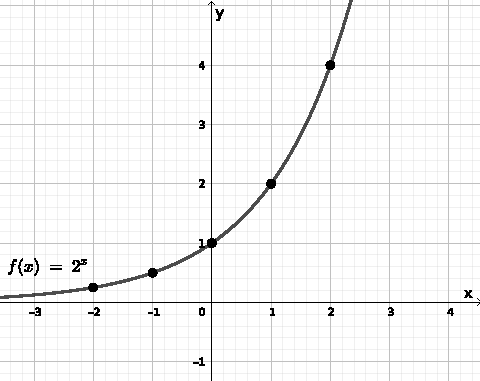
\includegraphics[width=7cm]{Capitulos/Figuras/f(x)=2^x.pdf}}
    \caption{Gráficos da função $f(x)=2^x$}
  \end{figure}

  Observe que neste caso a função é crescente, veremos que sempre que $1< a$ a função exponencial $f(x)=a^x$ será crescente e seu gráfico será parecido com este.

 \end{exem}


  \begin{exem}\label{ex:exp-1/2}
  Considere a função $f: \R \rightarrow \R_{+}^{*} $ dada por,
  \[f(x) = \left(\dfrac{1}{2}\right)^x \ , \]
  vamos determinar alguns pontos do gráfico da função $f$.

  \begin{table}[H]
  \centering
  \begin{tabular}{|c|c|c|} \hline
  \rowcolor{cinza}
  $x$ & $f(x) = \left(\dfrac{1}{2}\right)^x$ & $y$ \\ \hline
  $-2$ & $f(-2)= \left(\dfrac{1}{2}\right)^{-2}= 2^2$ & $4$ \\ \hline
  $-1$ & $f(-1)= \left(\dfrac{1}{2}\right)^{-1}= 2^1$ & $2$ \\ \hline
  $0$ & $f(0)= \left(\dfrac{1}{2}\right)^{0}$ & $1$ \\ \hline
  $1$ & $f(1)= \left(\dfrac{1}{2}\right)^{1}$ & $\dfrac{1}{2}$ \\ \hline
  $2$ & $f(2)= \left(\dfrac{1}{2}\right)^{2}$ & $\dfrac{1}{4}$ \\ \hline
  \end{tabular}
  \end{table}

  Marcando estes pontos no plano cartesiano e ligando obtemos o seguinte gráfico para esta função.

  \begin{figure}[H]
  \centering
    \fbox{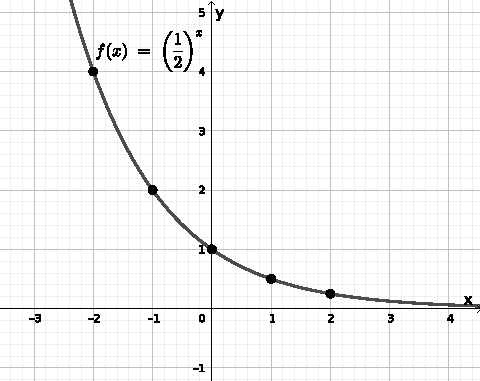
\includegraphics[width=7cm]{Capitulos/Figuras/f(x)=0_5^x.pdf}}
    \caption{Gráficos da função $f(x)=\left(\dfrac{1}{2}\right)^x$}
  \end{figure}

  Observe que neste caso a função é decrescente, veremos que sempre que $0< a < 1$ a função exponencial $f(x)=a^x$ será decrescente e seu gráfico será parecido com este.

 \end{exem}

 Para facilitar a comparação dos gráficos das funções dos dois últimos exemplos observe o plano cartesiano abaixo no qual temos os dois gráficos, note que eles são simétricos em relação ao eixo $y$.

   \begin{figure}[H]
 \centering
    \fbox{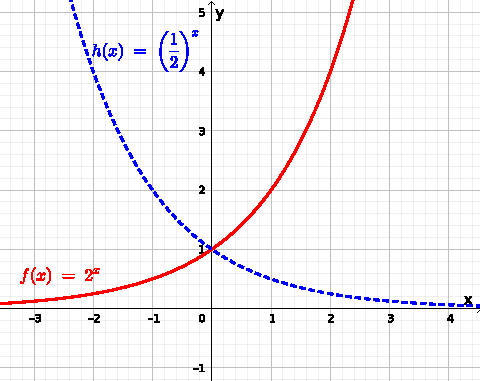
\includegraphics[width=8cm]{Capitulos/Figuras/comparandoexponenciais.pdf}}
    \caption{Comparando gráficos de funções exponenciais}
  \end{figure}


  \begin{exem} \label{ex:exp-e}
  Um caso especial de função exponencial é quando $a= e$, assim $f: \mathbb{R} \rightarrow \R_{+}^{*} $ será dada por:
  \[f(x) = e^x\]
  como $e= 2,7182818 \cdots$ decorre que $1 < e$ logo esta função é uma função crescente, e seu gráfico é:

  \begin{figure}[H]
 \centering
    \fbox{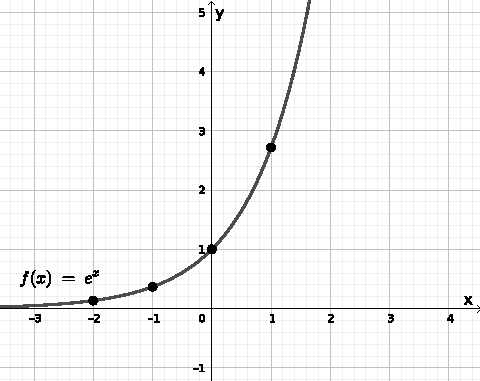
\includegraphics[width=7cm]{Capitulos/Figuras/f(x)=e^x.pdf}}
    \caption{Gráficos da função $f(x)= e^x$}
  \end{figure}
  \end{exem}

 \textbf{Propriedades:} Sejam $a, b \in \R_{+}^{*} \setminus \{1\}$ e $x, y \in \R$, nestas condições as seguintes propriedades são satisfeitas:
 \begin{enumerate}
  \item $a^x a^y= a^{x+y}$;
  \item $(a^x)^y= a^{xy}$;
  \item $(ab)^x= a^x b^x$;
  \item Se $0 < a < 1$ e $x < y$, então $a^x > a^y$, logo a função $f(x)= a^x$ é decrescente.
  \item Se $1 < a$ e $x < y$, então $a^x > a^y$, logo a função $f(x)= a^x$ é crescente.
 \end{enumerate}

 De (4) obtemos que $f(x)= a^x$, $a > 1$, é estritamente crescente em $\R$. De (5) obtemos que $f(x)= a^x$, $0 < a < 1$, é estritamente decrescente em $\R$. Portanto $\forall a > 0$ e $a \neq 1$ temos que a função exponencial $f(x)= a^x$ é bijetora.

 Além destas são válidas aqui também todas as propriedades de potências que já são conhecidas do leitor.


 \section{Funções logarítmicas}

 \colorbox{azul}{
 \begin{minipage}{0.9\linewidth}
 \begin{center}
 São funções $f: \mathbb{R_{+}^{*}} \rightarrow \mathbb{R} $ tais que:
 \[f(x) = \log_{a}(x)\]
 onde é dado $a \in \mathbb{R}$ satisfazendo $0 < a$ e $a \neq 1$. Estas funções são denominadas funções logarítmicas de base $a$.
 \end{center}
 \end{minipage}}

 \vskip0.3cm


 Observemos que dado um número real $a> 0$ e $a \neq 1$, para cada $y>0$ existe um único número real $x$ tal que $a^x= y$, já que como visto anteriormente a função exponencial $f(x)= a^x$ é bijetiva. Podemos assim definir o logaritmo de $y$ na base $a$ como sendo o número real $x$ tal que $a^x= y$. Simbolicamente,
 \[\destaque{\log_a(y)= x  \Leftrightarrow a^x= y}.\]

 Portanto, as funções logarítmica e exponencial são inversas uma da outra.

 \begin{exem} \label{ex:log-2}
  Considere a função $h: \mathbb{R_{+}^{*}} \rightarrow \mathbb{R} $ tais que:
 \[h(x) = \log_{2}(x) \ .\]
 Vamos encontrar alguns pontos do gráfico da função $h$.

  \begin{table}[H]
 \centering
 \begin{tabular}{|c|c|c|c|} \hline
 \rowcolor{cinza}
 $x$ & $h(x) = \log_{2}(x)$ & $y$ \\ \hline
 $\dfrac{1}{8}$ & $h\left(\dfrac{1}{8}\right)= \log_{2}\left(\dfrac{1}{8}\right)$ & $-3$ \\ \hline
 $\dfrac{1}{4}$ & $h\left(\dfrac{1}{4}\right)= \log_{2}\left(\dfrac{1}{4}\right)$ & $-2$ \\ \hline
 $\dfrac{1}{2}$ & $h\left(\dfrac{1}{2}\right)= \log_{2}\left(\dfrac{1}{2}\right)$ & $-1$ \\ \hline
 $1$ & $h(1)= \log_{2}(1)$ & $0$ \\ \hline
 $2$ & $h(2)= \log_{2}(2)$ & $1$ \\ \hline
 $4$ & $h(4)= \log_{2}(4)$ & $2$ \\ \hline
 $8$ & $h(8)= \log_{2}(8)$ & $3$ \\ \hline
 \end{tabular}
 \end{table}

 \[\log_{2}\left(\dfrac{1}{8}\right)= y \Leftrightarrow 2^y= \dfrac{1}{8} \Leftrightarrow 2^y= 2^{-3} \Leftrightarrow y=-3\]
 \[\log_{2}\left(\dfrac{1}{4}\right)= y \Leftrightarrow 2^y= \dfrac{1}{4} \Leftrightarrow 2^y= 2^{-2} \Leftrightarrow y=-2\]
 \[\log_{2}\left(\dfrac{1}{2}\right)= y \Leftrightarrow 2^y= \dfrac{1}{2} \Leftrightarrow 2^y= 2^{-1} \Leftrightarrow y=-1\]
 \[\log_{2}(1)= y \Leftrightarrow 2^y= 1 \Leftrightarrow 2^y= 2^0 \Leftrightarrow y=0\]
 \[\log_{2}(2)= y \Leftrightarrow 2^y= 2 \Leftrightarrow 2^y= 2^1 \Leftrightarrow y=1\]
 \[\log_{2}(4)= y \Leftrightarrow 2^y= 4 \Leftrightarrow 2^y= 2^2 \Leftrightarrow y=2\]
 \[\log_{2}(8)= y \Leftrightarrow 2^y= 8 \Leftrightarrow 2^y= 2^3 \Leftrightarrow y=3\]

 \begin{figure}[H]
    \centering
    \fbox{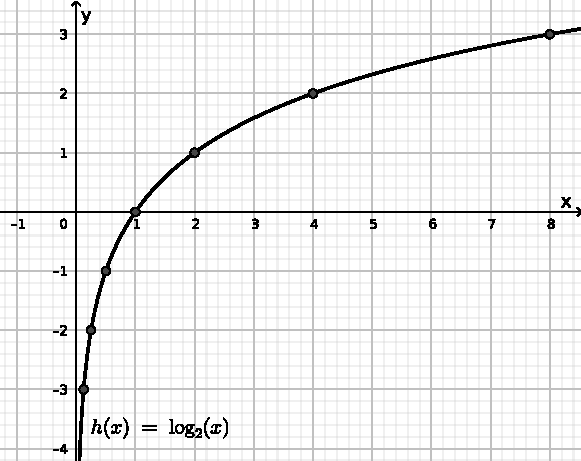
\includegraphics[width=7cm]{Capitulos/Figuras/h(x)=log_2.pdf}}
    \caption{Gráficos da função $h(x)= \log_{2}(x)$}
   \end{figure}
 Observe que a função $h(x)= \log_{2}(x)$ é estritamente crescente, veremos que sempre que $1< a$ a função $h(x)= \log_{a}(x)$ será estritamente crescente e seu gráfico será parecido com este.
 \end{exem}

 \begin{exem} \label{ex:log-1/2}
    Considere a função $h: \mathbb{R_{+}^{*}} \rightarrow \mathbb{R} $ tais que:
 \[h(x) = \log_{\frac{1}{2}}(x) \ .\]
 Vamos encontrar alguns pontos do gráfico da função $h$.

  \begin{table}[H]
 \centering
 \begin{tabular}{|c|c|c|c|} \hline
 \rowcolor{cinza}
 $x$ & $h(x) = \log_{\frac{1}{2}}(x)$ & $y$ \\ \hline
 $\dfrac{1}{8}$ & $h\left(\dfrac{1}{8}\right)= \log_{\frac{1}{2}}\left(\dfrac{1}{8}\right)$ & $3$ \\ \hline
 $\dfrac{1}{4}$ & $h\left(\dfrac{1}{4}\right)= \log_{\frac{1}{2}}\left(\dfrac{1}{4}\right)$ & $2$ \\ \hline
 $\dfrac{1}{2}$ & $h\left(\dfrac{1}{2}\right)= \log_{\frac{1}{2}}\left(\dfrac{1}{2}\right)$ & $1$ \\ \hline
 $1$ & $h(1)= \log_{\frac{1}{2}}(1)$ & $0$ \\ \hline
 $2$ & $h(2)= \log_{\frac{1}{2}}(2)$ & $-1$ \\ \hline
 $4$ & $h(4)= \log_{\frac{1}{2}}(4)$ & $-2$ \\ \hline
 $8$ & $h(8)= \log_{\frac{1}{2}}(8)$ & $-3$ \\ \hline
 \end{tabular}
 \end{table}

 \[\log_{\frac{1}{2}}\left(\dfrac{1}{8}\right)= y \Leftrightarrow \left(\dfrac{1}{2}\right)^y= \dfrac{1}{8} \Leftrightarrow \left(\dfrac{1}{2}\right)^y= \left(\dfrac{1}{2}\right)^{3} \Leftrightarrow y=3\]


 \begin{figure}[H]
    \centering
    \fbox{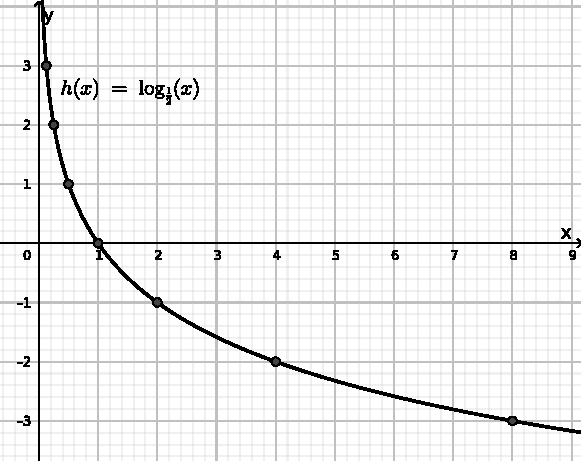
\includegraphics[width=7cm]{Capitulos/Figuras/h(x)=log_12.pdf}}
    \caption{Gráficos da função $h(x)= \log_{1/2}(x)$}
   \end{figure}
 Observe que a função $h(x)= \log_{1/2}(x)$ é estritamente decrescente, veremos que sempre que $0< a< 1$ a função $h(x)= \log_{a}(x)$ será decrescente e seu gráfico será parecido com este.
 \end{exem}

 Para facilitar a comparação dos gráficos das funções dos dois últimos exemplos observe o plano cartesiano abaixo no qual temos os dois gráficos, note que eles são simétricos em relação ao eixo $x$.

   \begin{figure}[H]
 \centering
    \fbox{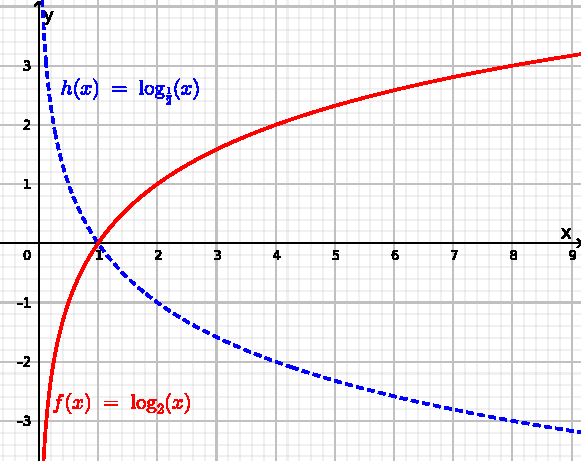
\includegraphics[width=8cm]{Capitulos/Figuras/comparandologs.pdf}}
    \caption{Comparando gráficos de funções logarítmicas}
  \end{figure}


  \begin{exem} \label{ex:log-e}
   Um caso especial de função logarítmica é quando $a= e$, assim $h: \mathbb{R_{+}^{*}} \rightarrow \mathbb{R} $ será dada por:
    \[h(x) = \log_{e}(x)= \ln(x)\]
  esta função é chamada logaritmo neperiano, que é uma função crescente, e seu gráfico é:

   \begin{figure}[H]
    \centering
    \fbox{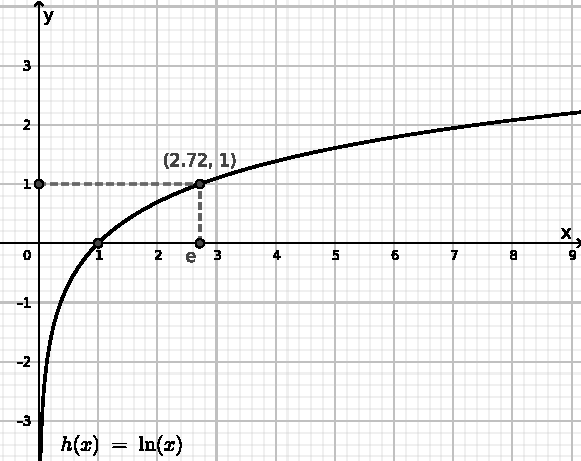
\includegraphics[width=7cm]{Capitulos/Figuras/f(x)=ln(x).pdf}}
    \caption{Gráficos da função $h(x)= \ln(x)$}
   \end{figure}

 \end{exem}

  \textbf{Propriedades:} Sejam $a, b \in \R_{+}^{*} \setminus \{1\}$, e $k$ uma constante real qualquer. Se $x, y \in \R_{+}^{*}$, então:

  \begin{enumerate}
  \item $\log_{a}(a)= 1$;
  \item $\log_{a}(1)= 0$;
   \item $\log_{a}(x \cdot y)=\log_{a}(x) + \log_{a}(y)$;
   \item $\log_{a} \left(\frac{x}{y}\right)=\log_{a}(x) - \log_{a}(y)$;
   \item $\log_{a}(x^{k})= k \log_{a}(x)$;
   \item $\log_{a}(a^n)= n$;
   \item (Mudança de base) \[\log_{a}(x)=\frac{\log_{b}(x)}{\log_{b}(a)};\]
   \item Se $0 < a < 1$ e $x < y$, então $\log_{a}(x) > \log_{a}(y)$, logo a função $h(x)= \log_{a}(x)$ é decrescente;
   \item Se $a> 1$ e $x < y$, então $\log_{a}(x) < \log_{a}(y)$, logo a função $h(x)= \log_{a}(x)$ é crescente.
  \end{enumerate}

  Vamos agora demonstrar algumas destas propriedades.

  \textbf{Propriedade 1:} $\log_{a}(a)= 1$, note que:
  \[\log_{a}(a)= y \Leftrightarrow a^y = a \Leftrightarrow a^y= a^1 \Leftrightarrow y=1\]
  \fim

  \textbf{Propriedade 2:} $\log_{a}(1)= 0$, note que:
  \[\log_{a}(1)= y \Leftrightarrow a^y= 1 \Leftrightarrow a^y= a^0 \Leftrightarrow y=0\]
  \fim

  \textbf{Propriedade 3:} $\log_{a}(x \cdot y)=\log_{a}(x) + \log_{a}(y)$, para tal definimos:
  \begin{eqnarray*}
   a^b= x & \Leftrightarrow & b= \log_{a}(x) \\
   a^c= y & \Leftrightarrow & c= \log_{a}(y) \\
   a^{b+c}= z & \Leftrightarrow & b+c= \log_{a}(z)
  \end{eqnarray*}
  com isso obtemos que
  \[x \cdot y= a^b \cdot a^c= a^{b+c}= z\]
  portanto,
  \[b+c= \log_{a}(z) \Rightarrow \log_{a}(x) + \log_{a}(y)= \log_{a}(x \cdot y)\]
  \fim

  \textbf{Propriedade 4:} $\log_{a} \left(\frac{x}{y}\right)=\log_{a}(x) - \log_{a}(y)$, para tal definimos:
  \begin{eqnarray*}
   a^b= x & \Leftrightarrow & b= \log_{a}(x) \\
   a^c= y & \Leftrightarrow & c= \log_{a}(y) \\
   a^{b-c}= z & \Leftrightarrow & b-c= \log_{a}(z)
  \end{eqnarray*}
  com isso obtemos que
  \[\dfrac{x}{y}= \dfrac{a^b}{a^c}= a^{b-c}= z\]
  portanto,
  \[b-c= \log_{a}(z) \Rightarrow \log_{a}(x) - \log_{a}(y)= \log_{a}\left(\frac{x}{y}\right)\]
  \fim

  \textbf{Propriedade 5:} $\log_{a}(x^k)= k \log_{a}(x)$, note que,
  \[\log_{a}(x^k)= \log_{a}\underbrace{(x \cdot x \cdots x)}_{k-vezes}= \underbrace{log_{a}(x) + log_{a}(x)+ \cdots + log_{a}(x)}_{k-vezes}= k \cdot log_{a}(x)\]
  \fim

  \textbf{Propriedade 6:} $\log_{a}(a^n)= n$, note que:
  \[\log_{a}(a^n)= n \cdot \log_{a}(a)= n \cdot 1 = n\]
  \fim

  Anteriormente comentamos que a função exponencial de base $a$ tem como inversa a função logaritmo de base $a$, vamos agora retomar os exemplos que fizemos acima, para comparar os gráficos das exponenciais com seus respectivos logaritmos inversos. Vamos com isso observar que em todos os casos os gráficos são simétricos em relação ao gráfico da função identidade $Id(x)= x$.

  \begin{enumerate}
   \item Considere o \autoref{ex:exp-2} e o \autoref{ex:log-2}. Nestes exemplos apresentamos as funções $f(x)= 2^x$ e $h(x)= \log_{2}(x)$ respectivamente, cujos gráficos são simétricos em relação ao gráfico da função $Id$, como pode ser visto na figura abaixo, isso ocorre pois as funções $f$ e $h$ são inversas uma da outra.

   \begin{figure}[H]
    \centering
    \fbox{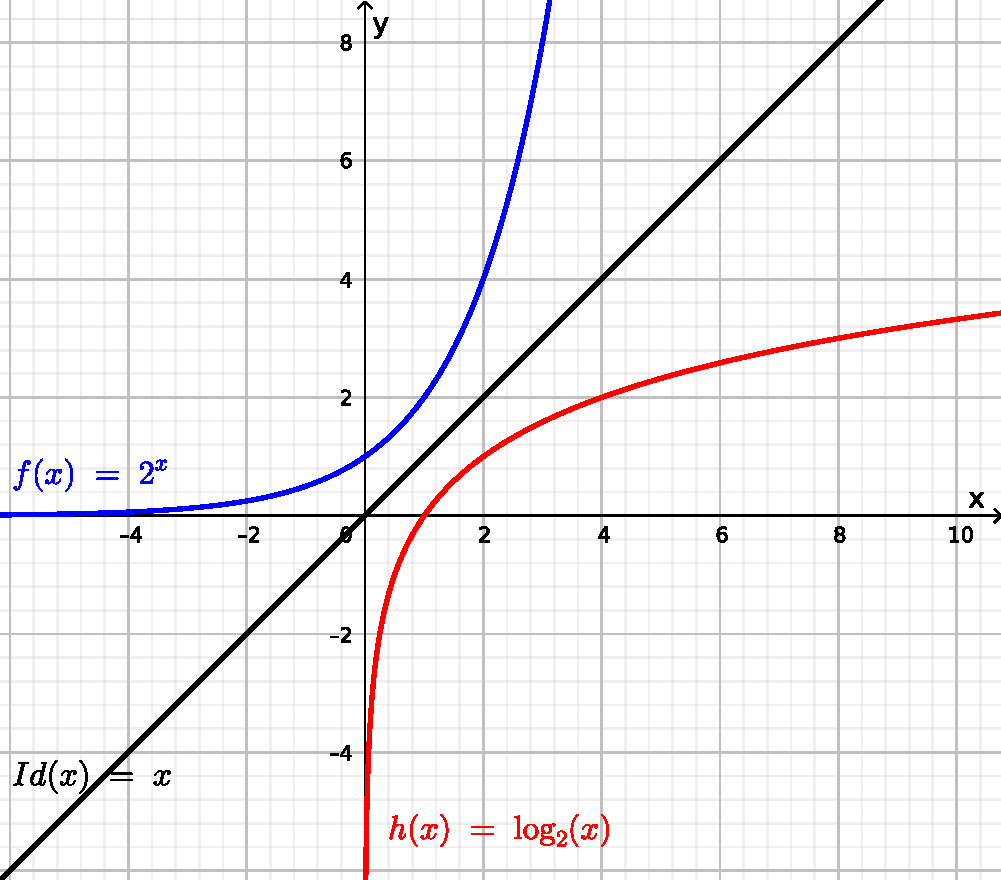
\includegraphics[width=9cm]{Capitulos/Figuras/comparandobase2.pdf}}
    \caption{Gráficos das funções exp e log de base $2$}
   \end{figure}

   \item Considere os exemplos \autoref{ex:exp-1/2} e \autoref{ex:log-1/2}, nestes exemplos apresentamos as funções $f(x)= \left(\frac{1}{2}\right)^x$ e $h(x)= \log_{\frac{1}{2}}(x)$ respectivamente, cujos gráficos são simétricos em relação ao gráfico da função $Id$, como pode ser visto na figura abaixo, isso ocorre pois as funções $f$ e $h$ são inversas uma da outra.

   \begin{figure}[H]
    \centering
    \fbox{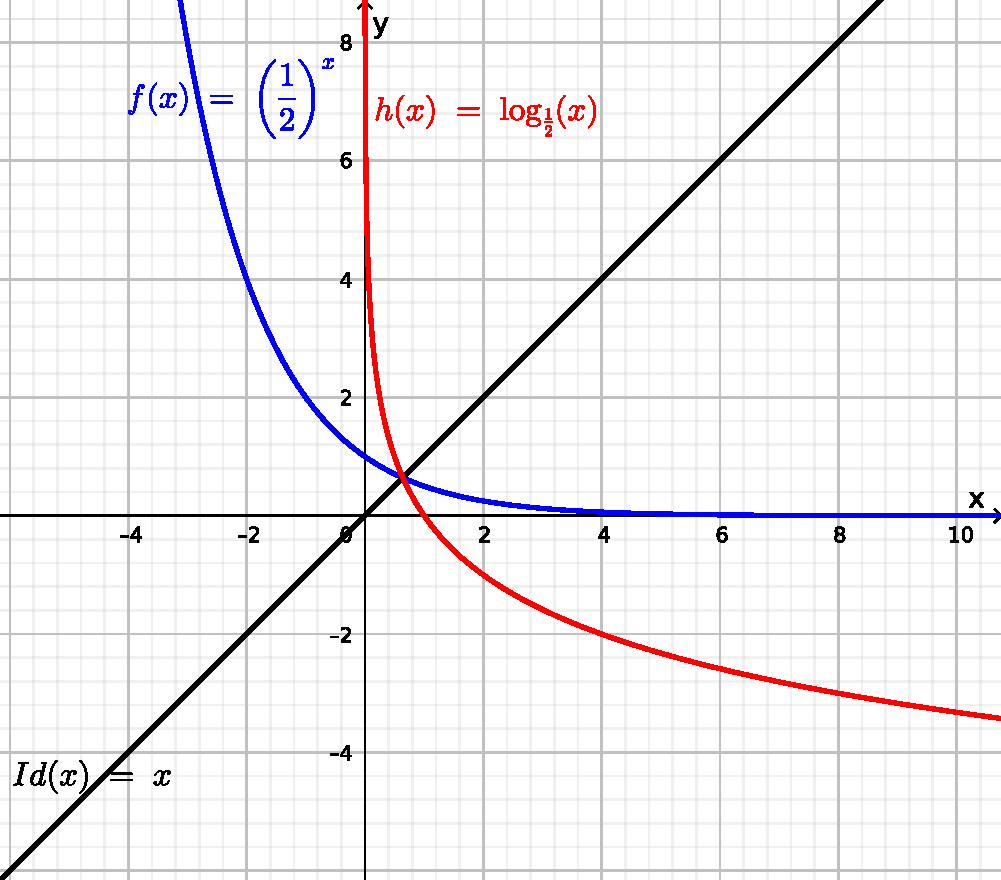
\includegraphics[width=9cm]{Capitulos/Figuras/comparandobase1-2.pdf}}
    \caption{Gráficos das funções exp e log de base $\frac{1}{2}$}
   \end{figure}

   \item Considere os exemplos \autoref{ex:exp-e} e \autoref{ex:log-e}, nestes exemplos apresentamos as funções $f(x)= e^x$ e $h(x)= \ln(x)$ respectivamente, cujos gráficos são simétricos em relação ao gráfico da função $Id$, como pode ser visto na figura abaixo, isso ocorre pois as funções $f$ e $h$ são inversas uma da outra.

   \begin{figure}[H]
    \centering
    \fbox{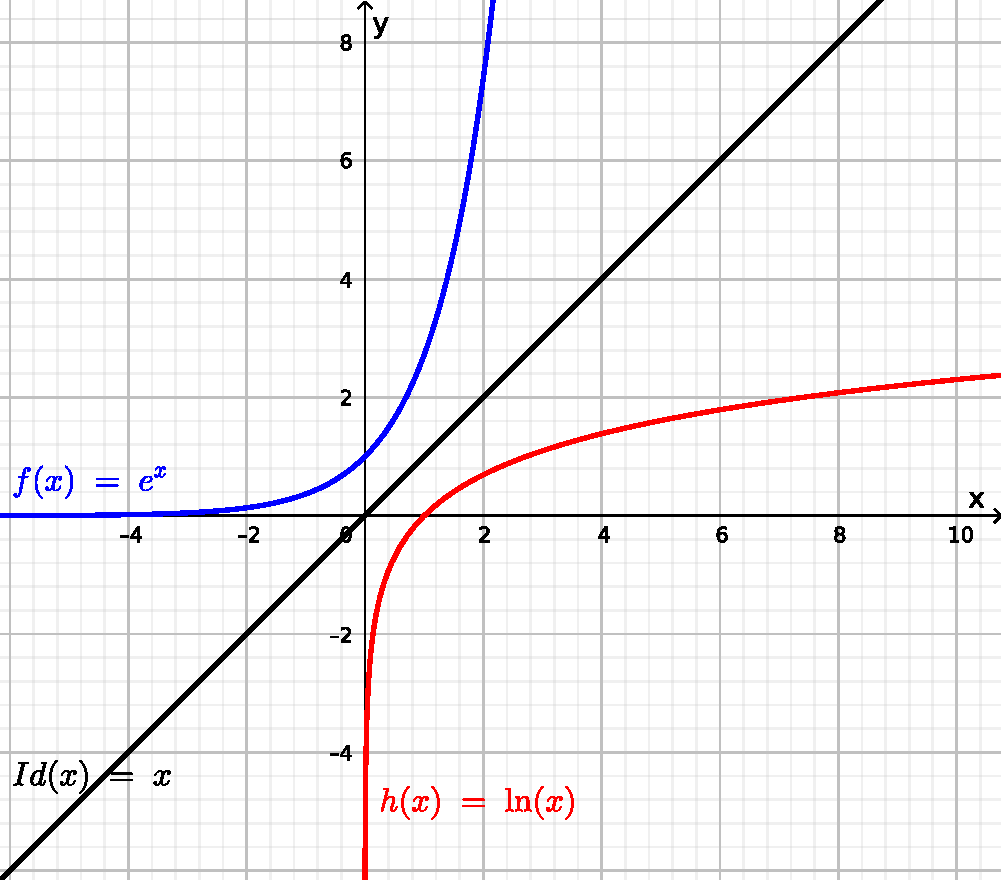
\includegraphics[width=9cm]{Capitulos/Figuras/comparandobase-e.pdf}}
    \caption{Gráficos das funções exp e log de base $e$}
   \end{figure}

  \end{enumerate}
  
